\subsection{UDP / TCP}
\label{udptcp:measure}
To analyse the power consumption while sending data to a server we prepared an 
experiment where we periodically sent data over TCP and UDP.\\

\subsubsection{Experimental setup}
To measure the current consumption, we used the setup from Fig. \ref{fig:experiment_setup} 
with the optional trigger.
The reason for this trigger is that the ESP8266-01 iteratively checks the connection to the access point when it is idle.
To distinguish between checking the connection and transmitting data, we trace the transmission process.
In order to analyze the power consumption when sending data via UDP,
we prepared a function that transfers data from an ESP8266-01 to the server.
To study the power consumption of TCP,
we sent data to a client over TCP using the ESP8266WiFi library. In our experiment, we sent random packets.
We then processed 100 cycles of the function in Fig. \ref{fig:tcp_uml} to gather enough values.
\newline
\begin{figure}[H]
\centering
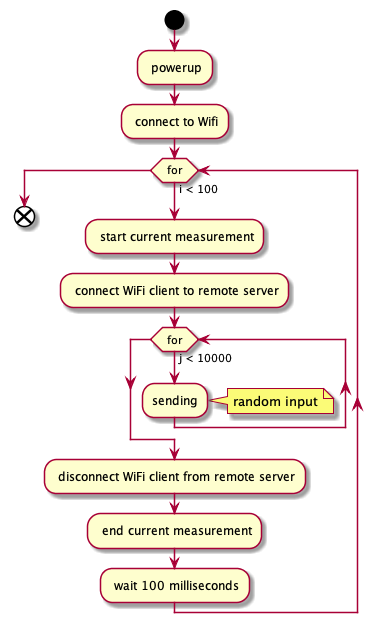
\includegraphics[width = 0.7 \linewidth]{fig/udp_tcp/tcp_uml.png}
\caption{Process to sending data over TCP}
\label{fig:tcp_uml}
\end{figure}
As expected, when we sent data over TCP, we got a lot of different results.
This is because TCP waits for the recipients response to send the data. \cite{postel1981transmission}
\newline
\begin{table}[htbp]
\begin{center}
\caption{Results TCP}
\label{tab:table1}
\renewcommand{\arraystretch}{1.8}
\begin{tabular}{l|c|r}
& \textbf{time [ms]} & \textbf{As}\\
\hline
count & 100 & 100\\
mean & 241.570 & 0.021031\\
std & 32.115403 & 0.002591\\
min & 193 & 0.016300\\
25\%  & 219 & 0.019175\\
50\% & 236 & 0.020600\\
75\%  & 257 & 0.022325\\
max & 396 & 0.032600\\
\end{tabular}
\end{center}
\end{table}
\newline
If we look at the results, we see that the current fluctuates a lot,
this is because TCP is monitoring the transmission 
and waits for the recipient to receive the packet.
\newline
\begin{figure}[H]
\centering
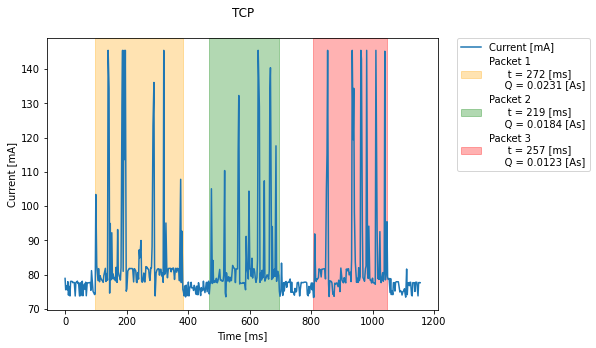
\includegraphics[width = 1 \linewidth]{fig/udp_tcp/tcp_s_m.png}
\caption{Sending data over TCP}
\label{fig:tcp_s_m}
\end{figure}

According to this, also the elapsed time is $236 \pm 13.63\% ms$
\linebreak
\begin{figure}[H]
\centering
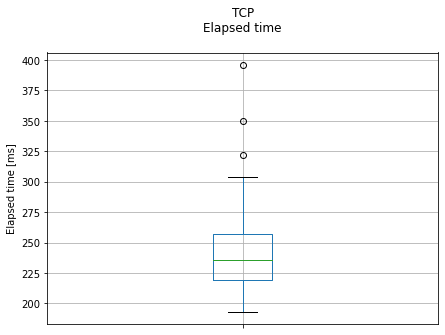
\includegraphics[width = 0.7 \linewidth]{fig/udp_tcp/tcp_boxplot_time.png}
\caption{Elapsed time while sending over TCP}
\label{fig:tcp_boxplot_time}
\end{figure}
In addition, the power consumption is $0.0206 \pm 12.58\% As$
\linebreak
\begin{figure}[H]
\centering
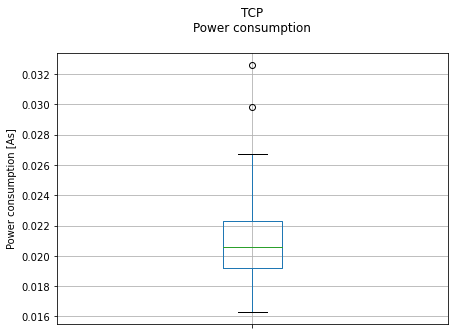
\includegraphics[width = 0.7 \linewidth]{fig/udp_tcp/tcp_boxplot_As.png}
\caption{Power consumption while sending over TCP}
\label{fig:tcp_boxplot_As}
\end{figure}
\subsubsection{UDP}
To analyse the power consumption while sending data over UDP we prepared a procedure which
transfers data from an ESP8266-01 to a server. For this, we used the WiFiUdp library.
In order to be able to compare with TCP, we create the process in Fig.\ref{fig:udp_uml}.
\linebreak\
\begin{figure}[H]
\centering
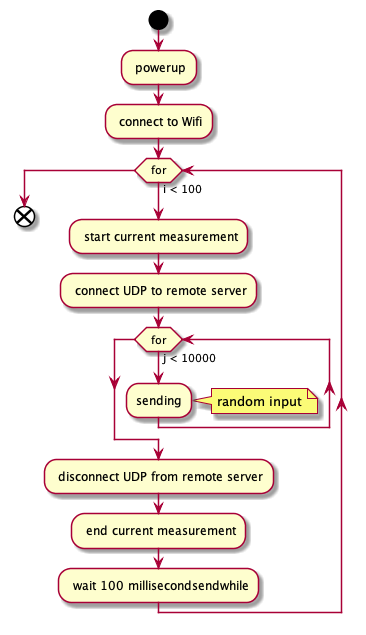
\includegraphics[width = 0.7 \linewidth]{fig/udp_tcp/udp_uml.png}
\caption{Process to send data over UDP}
\label{fig:udp_uml}
\end{figure}
As expected, when we sent data over UDP, we got more uniform values.
\linebreak\linebreak
\begin{table}[H]
\begin{center}
\caption{Results UDP}
\label{tab:table2}
\renewcommand{\arraystretch}{1.8}
\begin{tabular}{l|c|r}
& \textbf{time [ms]} & \textbf{As}\\
\hline
count & 100 & 100\\
mean & 95.970 & 0.009227\\
std & 1.058444 & 0.000581\\
min & 94 & 0.008200\\
25\% & 95 & 0.008800\\
50\% & 96 & 0.009100\\
75\% & 97 & 0.009600\\
max & 98 & 0.010900\\
\end{tabular}
\end{center}
\end{table}
If we look at the results, we see that the current is almost stable.
This is because UDP is not waiting for the recipient to receive the packet.
When it starts, it sends the packages simultaneously.\linebreak\linebreak
\begin{figure}[H]
\centering
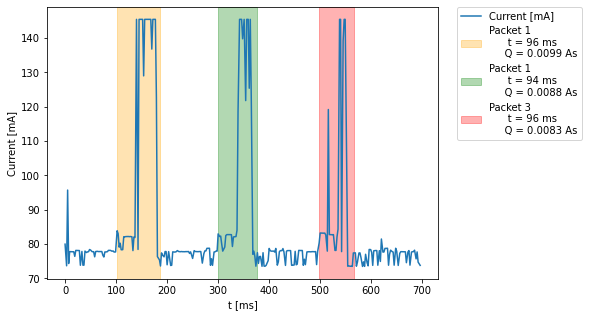
\includegraphics[width = 1 \linewidth]{fig/udp_tcp/udp_s_m.png}
\caption{Sending data over UDP}
\label{fig:udp_s_m}
\end{figure}
Accordingly, the elapsed time is $96 \pm 1.10\% ms$
\linebreak
\begin{figure}[H]
\centering
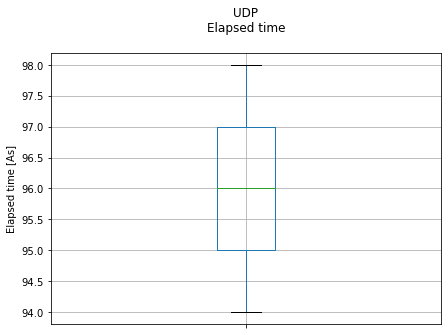
\includegraphics[width = 0.7 \linewidth]{fig/udp_tcp/udp_boxplot_time.png}
\caption{Elapsed time while sending over UDP}
\label{fig:udp_boxplot_time}
\end{figure}
In addition, the power consumption is $0.0091 \pm 6.38\% As$
\linebreak
\begin{figure}[H]
\centering
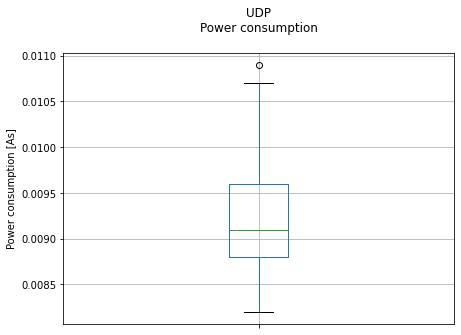
\includegraphics[width = 0.7 \linewidth]{fig/udp_tcp/udp_boxplot_As.png}
\caption{Power consumption while sending over UDP}
\label{fig:udp_boxplot_As}
\end{figure}